% !TeX spellcheck = hu_HU
% !TeX encoding = UTF-8
% !TeX program = xelatex
% TODO Change language to en_GB (recommended) or en_US for English documents
%\documentclass[11pt,a4paper,oneside]{report}             % Single-side
\documentclass[11pt,a4paper,twoside,openright]{report}  % Duplex

% thanks to http://tex.stackexchange.com/a/47579/71109
\usepackage{ifxetex}
\usepackage{ifluatex}
\newif\ifxetexorluatex % a new conditional starts as false
\ifnum 0\ifxetex 1\fi\ifluatex 1\fi>0
   \xetexorluatextrue
\fi

\ifxetexorluatex
  \usepackage{fontspec}
\else
  \usepackage[T1]{fontenc}
  \usepackage[utf8]{inputenc}
  \usepackage[lighttt]{lmodern}
\fi

\usepackage[english,magyar]{babel} % Alapértelmezés szerint utoljára definiált nyelv lesz aktív, de később külön beállítjuk az aktív nyelvet.

%\usepackage{cmap}
\usepackage{amsfonts,amsmath,amssymb} % Mathematical symbols.
%\usepackage[ruled,boxed,resetcount,linesnumbered]{algorithm2e} % For pseudocodes. % beware: this is not compatible with LuaLaTeX, see http://tex.stackexchange.com/questions/34814/lualatex-and-algorithm2e
\usepackage{booktabs} % For publication quality tables for LaTeX
\usepackage{graphicx}

%\usepackage{fancyhdr}
%\usepackage{lastpage}

\usepackage{anysize}
%\usepackage{sectsty}
\usepackage{setspace} % For setting line spacing

\usepackage[unicode]{hyperref} % For hyperlinks in the generated document.
\usepackage{xcolor}
\usepackage{listings} % For source code snippets.

\usepackage[amsmath,thmmarks]{ntheorem} % Theorem-like environments.

\usepackage[hang]{caption}

\singlespacing

\newcommand{\selecthungarian}{
	\selectlanguage{magyar}
	\setlength{\parindent}{2em}
	\setlength{\parskip}{0em}
	\frenchspacing
}

\newcommand{\selectenglish}{
	\selectlanguage{english}
	\setlength{\parindent}{0em}
	\setlength{\parskip}{0.5em}
	\nonfrenchspacing
	\renewcommand{\figureautorefname}{Figure}
	\renewcommand{\tableautorefname}{Table}
	\renewcommand{\partautorefname}{Part}
	\renewcommand{\chapterautorefname}{Chapter}
	\renewcommand{\sectionautorefname}{Section}
	\renewcommand{\subsectionautorefname}{Section}
	\renewcommand{\subsubsectionautorefname}{Section}
}

\usepackage[numbers]{natbib}
\usepackage{xspace}


%TODO Set the main variables
\newcommand{\vikszerzoVezeteknev}{Kunkli}
\newcommand{\vikszerzoKeresztnev}{Richárd}

\newcommand{\vikkonzulensAMegszolitas}{dr.~}
\newcommand{\vikkonzulensAVezeteknev}{Simon}
\newcommand{\vikkonzulensAKeresztnev}{Csaba}

\newcommand{\vikkonzulensBMegszolitas}{}
\newcommand{\vikkonzulensBVezeteknev}{}
\newcommand{\vikkonzulensBKeresztnev}{}

\newcommand{\vikkonzulensCMegszolitas}{}
\newcommand{\vikkonzulensCVezeteknev}{}
\newcommand{\vikkonzulensCKeresztnev}{}

\newcommand{\vikcim}{Vizualizációs megoldás IoT adat elemző rendszerhez} % Cím
\newcommand{\viktanszek}{\bmetmit} % Tanszék
\newcommand{\vikdoktipus}{\bsc} % Dokumentum típusa (\bsc vagy \msc)
\newcommand{\vikmunkatipusat}{szakdolgozatot} % a "hallgató nyilatkozat" részhez: szakdolgozatot vagy diplomatervet

%--------------------------------------------------------------------------------------
% TDK-specifikus változók
%--------------------------------------------------------------------------------------
\newcommand{\tdkszerzoB}{Második Szerző} % Második szerző neve; hagyd üresen, ha egyedül írtad a TDK-t.
\newcommand{\tdkev}{2014} % A dolgozat írásának éve (pl. "2014") (Ez OTDK-nál eltérhet az aktuális évtől.)

% További adatok az OTDK címlaphoz (BME-s TDK-hoz nem kell kitölteni)
\newcommand{\tdkevfolyamA}{IV} % Első szerző évfolyama, római számmal (pl. IV).
\newcommand{\tdkevfolyamB}{III} % Második szerző évfolyama, római számmal (pl. III).
\newcommand{\tdkkonzulensbeosztasA}{egyetemi tanár} % Első konzulens beosztása (pl. egyetemi docens)
\newcommand{\tdkkonzulensbeosztasB}{doktorandusz} % Második konzulens beosztása (pl. egyetemi docens)

\newcommand{\szerzoMeta}{\vikszerzoVezeteknev{} \vikszerzoKeresztnev} % egy szerző esetén
%\newcommand{\szerzoMeta}{\vikszerzoVezeteknev{} \vikszerzoKeresztnev, \tdkszerzoB} % két szerző esetén

%TODO Language configuration -- choose one
% Beállítások magyar nyelvű dolgozathoz
%--------------------------------------------------------------------------------------
% Elnevezések
%--------------------------------------------------------------------------------------
\newcommand{\bme}{Budapesti Műszaki és Gazdaságtudományi Egyetem}
\newcommand{\vik}{Villamosmérnöki és Informatikai Kar}

\newcommand{\bmemit}{Méréstechnika és Információs Rendszerek Tanszék}

\newcommand{\keszitette}{Készítette}
\newcommand{\konzulens}{Konzulens}

\newcommand{\bsc}{Szakdolgozat}
\newcommand{\msc}{Diplomaterv}
\newcommand{\tdk}{TDK dolgozat}
\newcommand{\bsconlab}{BSc Önálló laboratórium}
\newcommand{\msconlabi}{MSc Önálló laboratórium 1.}
\newcommand{\msconlabii}{MSc Önálló laboratórium 2.}

\newcommand{\pelda}{Példa}
\newcommand{\definicio}{Definíció}
\newcommand{\tetel}{Tétel}

\newcommand{\bevezetes}{Bevezetés}
\newcommand{\koszonetnyilvanitas}{Köszönetnyilvánítás}
\newcommand{\fuggelek}{Függelék}

% Opcionálisan átnevezhető címek
%\addto\captionsmagyar{%
%\renewcommand{\listfigurename}{Saját ábrajegyzék cím}
%\renewcommand{\listtablename}{Saját táblázatjegyzék cím}
%\renewcommand{\bibname}{Saját irodalomjegyzék név}
%}

\newcommand{\szerzo}{\vikszerzoVezeteknev{} \vikszerzoKeresztnev}
\newcommand{\vikkonzulensA}{\vikkonzulensAMegszolitas\vikkonzulensAVezeteknev{} \vikkonzulensAKeresztnev}
\newcommand{\vikkonzulensB}{\vikkonzulensBMegszolitas\vikkonzulensBVezeteknev{} \vikkonzulensBKeresztnev}
\newcommand{\vikkonzulensC}{\vikkonzulensCMegszolitas\vikkonzulensCVezeteknev{} \vikkonzulensCKeresztnev}

\newcommand{\selectthesislanguage}{\selecthungarian}

\bibliographystyle{huplain}

\def\lstlistingname{lista}

\newcommand{\appendixnumber}{6}  % a fofejezet-szamlalo az angol ABC 6. betuje (F) lesz

% Settings for English documents
%%--------------------------------------------------------------------------------------
% Elnevezések
%--------------------------------------------------------------------------------------
\newcommand{\bme}{Budapest University of Technology and Economics}
\newcommand{\vik}{Faculty of Electrical Engineering and Informatics}

\newcommand{\bmemit}{Department of Measurement and Information Systems}

\newcommand{\keszitette}{Author}
\newcommand{\konzulens}{Advisor}

\newcommand{\bsc}{Bachelor's Thesis}
\newcommand{\msc}{Master's Thesis}
\newcommand{\tdk}{Scientific Students' Association Report}
\newcommand{\bsconlab}{BSc Project Laboratory}
\newcommand{\msconlabi}{MSc Project Laboratory 1}
\newcommand{\msconlabii}{MSc Project Laboratory 2}

\newcommand{\pelda}{Example}
\newcommand{\definicio}{Definition}
\newcommand{\tetel}{Theorem}

\newcommand{\bevezetes}{Introduction}
\newcommand{\koszonetnyilvanitas}{Acknowledgements}
\newcommand{\fuggelek}{Appendix}

% Optional custom titles
%\addto\captionsenglish{%
%\renewcommand*{\listfigurename}{Your list of figures title}
%\renewcommand*{\listtablename}{Your list of tables title}
%\renewcommand*{\bibname}{Your bibliography title}
%}

\newcommand{\szerzo}{\vikszerzoKeresztnev{} \vikszerzoVezeteknev}
\newcommand{\vikkonzulensA}{\vikkonzulensAMegszolitas\vikkonzulensAKeresztnev{} \vikkonzulensAVezeteknev}
\newcommand{\vikkonzulensB}{\vikkonzulensBMegszolitas\vikkonzulensBKeresztnev{} \vikkonzulensBVezeteknev}
\newcommand{\vikkonzulensC}{\vikkonzulensCMegszolitas\vikkonzulensCKeresztnev{} \vikkonzulensCVezeteknev}

\newcommand{\selectthesislanguage}{\selectenglish}

\bibliographystyle{plainnat}

\newcommand{\ie}{i.e.\@\xspace}
\newcommand{\Ie}{I.e.\@\xspace}
\newcommand{\eg}{e.g.\@\xspace}
\newcommand{\Eg}{E.g.\@\xspace}
\newcommand{\etal}{et al.\@\xspace}
\newcommand{\etc}{etc.\@\xspace}
\newcommand{\vs}{vs.\@\xspace}
\newcommand{\viz}{viz.\@\xspace} % videlicet
\newcommand{\cf}{cf.\@\xspace} % confer
\newcommand{\Cf}{Cf.\@\xspace}
\newcommand{\wrt}{w.r.t.\@\xspace} % with respect to
\newcommand{\approximately}{approx.\@\xspace}

\newcommand{\appendixnumber}{1}  % a fofejezet-szamlalo az angol ABC 1. betuje (A) lesz


%--------------------------------------------------------------------------------------
% Page layout setup
%--------------------------------------------------------------------------------------
% we need to redefine the pagestyle plain
% another possibility is to use the body of this command without \fancypagestyle
% and use \pagestyle{fancy} but in that case the special pages
% (like the ToC, the References, and the Chapter pages)remain in plane style

\pagestyle{plain}
\marginsize{35mm}{25mm}{15mm}{15mm}

\setcounter{tocdepth}{3}
%\sectionfont{\large\upshape\bfseries}
\setcounter{secnumdepth}{3}

\sloppy % Margón túllógó sorok tiltása.
\widowpenalty=10000 \clubpenalty=10000 %A fattyú- és árvasorok elkerülése
\def\hyph{-\penalty0\hskip0pt\relax} % Kötőjeles szavak elválasztásának engedélyezése


%--------------------------------------------------------------------------------------
% Setup hyperref package
%--------------------------------------------------------------------------------------
\hypersetup{
    % bookmarks=true,            % show bookmarks bar?
    unicode=true,              % non-Latin characters in Acrobat's bookmarks
    pdftitle={\vikcim},        % title
    pdfauthor={\szerzoMeta},    % author
    pdfsubject={\vikdoktipus}, % subject of the document
    pdfcreator={\szerzoMeta},   % creator of the document
    pdfproducer={},    % producer of the document
    pdfkeywords={},    % list of keywords (separate then by comma)
    pdfnewwindow=true,         % links in new window
    colorlinks=true,           % false: boxed links; true: colored links
    linkcolor=black,           % color of internal links
    citecolor=black,           % color of links to bibliography
    filecolor=black,           % color of file links
    urlcolor=black             % color of external links
}


%--------------------------------------------------------------------------------------
% Set up listings
%--------------------------------------------------------------------------------------

\definecolor{red}{rgb}{0.6,0,0} 
\definecolor{blue}{rgb}{0,0,0.6}
\definecolor{lightblue}{rgb}{0,0.5,0.7}
\definecolor{green}{rgb}{0,0.8,0}
\definecolor{cyan}{rgb}{0.0,0.6,0.6}
\definecolor{orange}{rgb}{0.8,0.6,0}
\definecolor{white}{rgb}{0.98, 0.98, 0.98}
\definecolor{lightgray}{rgb}{0.95,0.95,0.95}
\definecolor{darkviolet}{rgb}{0.58, 0.0, 0.83}
\definecolor{royalblue}{rgb}{0.25, 0.41, 0.88}

\lstdefinestyle{csharp}{
	language=csh,
	basicstyle=\scriptsize\ttfamily,
	numbers=left,
	numberstyle=\tiny,
	numbersep=5pt,
	tabsize=2,
	extendedchars=true,
	breaklines=true,
	frame=b,
	stringstyle=\color{red}\ttfamily,
	showspaces=false,
	captionpos=b,
	showtabs=false,
	xleftmargin=17pt,
	framexleftmargin=17pt,
	framexrightmargin=5pt,
	framexbottommargin=4pt,
	commentstyle=\color{green},
	morecomment=[l]{//}, %use comment-line-style!
	morecomment=[s]{/*}{*/}, %for multiline comments
	showstringspaces=false,
	morekeywords={ abstract, event, new, struct,
		as, explicit, null, switch,
		base, extern, object, this,
		get, set,
		bool, false, operator, throw,
		break, finally, out, true,
		byte, fixed, override, try,
		case, float, params, typeof,
		catch, for, private, uint,
		char, foreach, protected, ulong,
		checked, goto, public, unchecked,
		class, record, async, if, readonly, unsafe,
		const, implicit, ref, ushort,
		continue, in, return, using,
		decimal, int, sbyte, virtual,
		default, interface, sealed, volatile,
		delegate, internal, short, void,
		do, is, sizeof, while,
		double, lock, stackalloc,
		else, long, static,
		enum, namespace, string},
	morekeywords=[2]{CreateMap, ForMember, MapFrom, ReverseMap, Onlineall, GetMapper, GetUserFromDb, Map},
	morekeywords=[3]{Id, Name, PasswordHash, PasswordSalt, Role, IsFromConfig, Url, Username, UserRole, mapper, user, response},
	keywordstyle=\color{blue},
	keywordstyle={[2]\color{orange}},
	keywordstyle={[3]\color{lightblue}},
	identifierstyle=\color{cyan},
	backgroundcolor=\color{white}
}

\lstdefinestyle{jsx}{
	basicstyle=\scriptsize\ttfamily,
	numbers=left,
	numberstyle=\tiny,
	numbersep=5pt,
	tabsize=2,
	extendedchars=true,
	breaklines=true,
	frame=b,
	stringstyle=\color{red}\ttfamily,
	showspaces=false,
	captionpos=b,
	showtabs=false,
	xleftmargin=17pt,
	framexleftmargin=17pt,
	framexrightmargin=5pt,
	framexbottommargin=4pt,
	commentstyle=\color{green},
	morestring=*[d]{"},
	morecomment=[l]{//}, %use comment-line-style!
	morecomment=[s]{/*}{*/}, %for multiline comments
	showstringspaces=false,
	morekeywords={ },
	morekeywords=[2]{AuthComponent, LogsComponent, DashboardComponent, DevicesComponent, HeatmapComponent},
	morekeywords=[3]{exact, path, component},
	keywordstyle=\color{blue},
	keywordstyle={[2]\color{orange}},
	keywordstyle={[3]\color{lightblue}},
	identifierstyle=\color{cyan},
	backgroundcolor=\color{white}
}
\lstdefinestyle{xml}{
	basicstyle=\scriptsize\ttfamily, % print whole listing small
	% default behavior: comments in italic, to change use
	% commentstyle=\color{green}, % for e.g. green comments
	showstringspaces=false, % no special string spaces
	aboveskip=3pt,
	belowskip=3pt,
	stringstyle=\color{red}\ttfamily,
	backgroundcolor=\color{white},
	keywordstyle=\color{blue},
	identifierstyle=\color{cyan},
	columns=flexible,
	keepspaces=true,
	escapeinside={(*@}{@*)},
	captionpos=b,
	breaklines=true,
	frame=b,
	float=!ht,
	tabsize=2,
	morestring=*[d]{"},
	morekeywords={targets, target, rules, logger},
	literate=*
		{á}{{\'a}}1	{é}{{\'e}}1	{í}{{\'i}}1	{ó}{{\'o}}1	{ö}{{\"o}}1	{ő}{{\H{o}}}1	{ú}{{\'u}}1	{ü}{{\"u}}1	{ű}{{\H{u}}}1
		{Á}{{\'A}}1	{É}{{\'E}}1	{Í}{{\'I}}1	{Ó}{{\'O}}1	{Ö}{{\"O}}1	{Ő}{{\H{O}}}1	{Ú}{{\'U}}1	{Ü}{{\"U}}1	{Ű}{{\H{U}}}1
}

%--------------------------------------------------------------------------------------
% Set up theorem-like environments
%--------------------------------------------------------------------------------------
% Using ntheorem package -- see http://www.math.washington.edu/tex-archive/macros/latex/contrib/ntheorem/ntheorem.pdf

\theoremstyle{plain}
\theoremseparator{.}
\newtheorem{example}{\pelda}

\theoremseparator{.}
%\theoremprework{\bigskip\hrule\medskip}
%\theorempostwork{\hrule\bigskip}
\theorembodyfont{\upshape}
\theoremsymbol{{\large \ensuremath{\centerdot}}}
\newtheorem{definition}{\definicio}

\theoremseparator{.}
%\theoremprework{\bigskip\hrule\medskip}
%\theorempostwork{\hrule\bigskip}
\newtheorem{theorem}{\tetel}


%--------------------------------------------------------------------------------------
% Some new commands and declarations
%--------------------------------------------------------------------------------------
\newcommand{\code}[1]{{\upshape\ttfamily\scriptsize\indent #1}}
\newcommand{\doi}[1]{DOI: \href{http://dx.doi.org/\detokenize{#1}}{\raggedright{\texttt{\detokenize{#1}}}}} % A hivatkozások közt így könnyebb DOI-t megadni.

\DeclareMathOperator*{\argmax}{arg\,max}
%\DeclareMathOperator*[1]{\floor}{arg\,max}
\DeclareMathOperator{\sign}{sgn}
\DeclareMathOperator{\rot}{rot}


%--------------------------------------------------------------------------------------
% Setup captions
%--------------------------------------------------------------------------------------
\captionsetup[figure]{
	width=.75\textwidth,
	aboveskip=10pt}

\renewcommand{\captionlabelfont}{\bf}
%\renewcommand{\captionfont}{\footnotesize\it}

%--------------------------------------------------------------------------------------
% Hyphenation exceptions
%--------------------------------------------------------------------------------------
\hyphenation{Shakes-peare Mar-seilles ár-víz-tű-rő tü-kör-fú-ró-gép}


\author{\vikszerzo}
\title{\viktitle}

%--------------------------------------------------------------------------------------
% Table of contents and the main text
%--------------------------------------------------------------------------------------
\begin{document}
\pagenumbering{gobble}

%TODO These includes define guidelines -- remove these
%~~~~~~~~~~~~~~~~~~~~~~~~~~~~~~~~~~~~~~~~~~~~~~~~~~~~~~~~~~~~~~~~~~~~~~~~~~~~~~~~~~~~~~
%\selecthungarian
%--------------------------------------------------------------------------------------
% Rovid formai es tartalmi tajekoztato
%--------------------------------------------------------------------------------------

\footnotesize
\begin{center}
\large
\textbf{\Large Általános információk, a diplomaterv szerkezete}\\
\end{center}

A diplomaterv szerkezete a BME Villamosmérnöki és Informatikai Karán:
\begin{enumerate}
\item	Diplomaterv feladatkiírás
\item	Címoldal
\item	Tartalomjegyzék
\item	A diplomatervező nyilatkozata az önálló munkáról és az elektronikus adatok kezeléséről
\item	Tartalmi összefoglaló magyarul és angolul
\item	Bevezetés: a feladat értelmezése, a tervezés célja, a feladat indokoltsága, a diplomaterv felépítésének rövid összefoglalása
\item	A feladatkiírás pontosítása és részletes elemzése
\item	Előzmények (irodalomkutatás, hasonló alkotások), az ezekből levonható következtetések
\item	A tervezés részletes leírása, a döntési lehetőségek értékelése és a választott megoldások indoklása
\item	A megtervezett műszaki alkotás értékelése, kritikai elemzése, továbbfejlesztési lehetőségek
\item	Esetleges köszönetnyilvánítások
\item	Részletes és pontos irodalomjegyzék
\item	Függelék(ek)
\end{enumerate}

Felhasználható a következő oldaltól kezdődő \LaTeX diplomatervsablon dokumentum tartalma. 

A diplomaterv szabványos méretű A4-es lapokra kerüljön. Az oldalak tükörmargóval készüljenek (mindenhol 2,5~cm, baloldalon 1~cm-es kötéssel). Az alapértelmezett betűkészlet a 12 pontos Times New Roman, másfeles sorközzel, de ettől kismértékben el lehet térni, ill. más betűtípus használata is megengedett.

Minden oldalon -- az első négy szerkezeti elem kivételével -- szerepelnie kell az oldalszámnak.

A fejezeteket decimális beosztással kell ellátni. Az ábrákat a megfelelő helyre be kell illeszteni, fejezetenként decimális számmal és kifejező címmel kell ellátni. A fejezeteket decimális aláosztással számozzuk, maximálisan 3 aláosztás mélységben (pl. 2.3.4.1.). Az ábrákat, táblázatokat és képleteket célszerű fejezetenként külön számozni (pl. 2.4. ábra, 4.2. táblázat vagy képletnél (3.2)). A fejezetcímeket igazítsuk balra, a normál szövegnél viszont használjunk sorkiegyenlítést. Az ábrákat, táblázatokat és a hozzájuk tartozó címet igazítsuk középre. A cím a jelölt rész alatt helyezkedjen el.

A képeket lehetőleg rajzoló programmal készítsék el, az egyenleteket egyenlet-szerkesztő segítségével írják le (A \LaTeX~ehhez kézenfekvő megoldásokat nyújt).

Az irodalomjegyzék szövegközi hivatkozása történhet sorszámozva (ez a preferált megoldás) vagy a Harvard-rendszerben (a szerző és az évszám megadásával). A teljes lista névsor szerinti sorrendben a szöveg végén szerepeljen (sorszámozott irodalmi hivatkozások esetén hivatkozási sorrendben). A szakirodalmi források címeit azonban mindig az eredeti nyelven kell megadni, esetleg zárójelben a fordítással. A listában szereplő valamennyi publikációra hivatkozni kell a szövegben (a \LaTeX-sablon a Bib\TeX~segítségével mindezt automatikusan kezeli). Minden publikáció a szerzők után a következő adatok szerepelnek: folyóirat cikkeknél a pontos cím, a folyóirat címe, évfolyam, szám, oldalszám tól-ig. A folyóiratok címét csak akkor rövidítsük, ha azok nagyon közismertek vagy nagyon hosszúak. Internetes hivatkozások megadásakor fontos, hogy az elérési út előtt megadjuk az oldal tulajdonosát és tartalmát (mivel a link egy idő után akár elérhetetlenné is válhat), valamint az elérés időpontját.

\vspace{5mm}
Fontos:
\begin{itemize}
	\item A szakdolgozatkészítő / diplomatervező nyilatkozata (a jelen sablonban szereplő szövegtartalommal) kötelező előírás, Karunkon ennek hiányában a szakdolgozat/diplomaterv nem bírálható és nem védhető!
	\item Mind a dolgozat, mind a melléklet maximálisan 15~MB méretű lehet!
\end{itemize}

\vspace{5mm}
\begin{center}
Jó munkát, sikeres szakdolgozatkészítést, ill. diplomatervezést kívánunk!
\end{center}

\normalsize
\selectthesislanguage

%%--------------------------------------------------------------------------------------
% Feladatkiiras (a tanszeken atveheto, kinyomtatott valtozat)
%--------------------------------------------------------------------------------------
\clearpage
\begin{center}
\large
\textbf{FELADATKIÍRÁS}\\
\end{center}

A feladatkiírást a tanszéki adminisztrációban lehet átvenni, és a leadott munkába eredeti, tanszéki pecséttel ellátott és a tanszékvezető által aláírt lapot kell belefűzni (ezen oldal \emph{helyett}, ez az oldal csak útmutatás). Az elektronikusan feltöltött dolgozatban már nem kell beleszerkeszteni ezt a feladatkiírást.


\selectthesislanguage

%TODO Titlepage -- choose one from below
%~~~~~~~~~~~~~~~~~~~~~~~~~~~~~~~~~~~~~~~~~~~~~~~~~~~~~~~~~~~~~~~~~~~~~~~~~~~~~~~~~~~~~~
\hypersetup{pageanchor=false}
%--------------------------------------------------------------------------------------
%	The title page
%--------------------------------------------------------------------------------------
\begin{titlepage}
\begin{center}

\includegraphics[width=60mm,keepaspectratio]{figures/bme_logo.pdf}\\
\vspace{0.3cm}
\textbf{\bme}\\
\textmd{\vik}\\
\textmd{\viktanszek}\\[5cm]

\vspace{0.4cm}
{\huge \bfseries \vikcim}\\[0.8cm]
\vspace{0.5cm}
\textsc{\Large \vikdoktipus}\\[4cm]

{
	\renewcommand{\arraystretch}{0.85}
	\begin{tabular}{cc}
	 \makebox[7cm]{\emph{\keszitette}} & \makebox[7cm]{\emph{\konzulens}} \\ \noalign{\smallskip}
	 \makebox[7cm]{\szerzo} & \makebox[7cm]{\vikkonzulensA} \\
	  & \makebox[7cm]{\vikkonzulensB} \\
	  & \makebox[7cm]{\vikkonzulensC} \\
	\end{tabular}
}

\vfill
{\large \today}
\end{center}
\end{titlepage}
\hypersetup{pageanchor=false}

		   % Szakdolgozat/Diplomaterv címlap
%%% TDK címlap
\begin{titlepage}
  \begin{center}  
  
\includegraphics[width=7cm]{./figures/bme_logo.pdf}
  \vspace{0.3cm}
  
  \bme \\
  \vik \\
  \viktanszek \\
  \vspace{5cm}
  
  \huge {\vikcim}
  \vspace{1.5cm}
  
  \large {\textbf{\tdk}}
  \vfill
    
  {\Large 
  	\keszitette: \\ \vspace{0.3cm}
  	\szerzo \\
	\tdkszerzoB \\
  	\vspace{1.5cm}
  	\konzulens: \\ \vspace{0.3cm}
  	\vikkonzulensA \\
  	\vikkonzulensB \\
  }
  
  \vspace{2cm}
  \large {\tdkev}
 \end{center}
\end{titlepage}
%% Címlap vége
	% TDK címlap
%%% OTDK külső címlap
\begin{titlepage}
  	$\;$ 
	\vspace{5cm}
	
	\begin{center}
	\Huge
	\textbf{TDK-dolgozat}\let\thefootnote\relax\footnote{A dolgozat bemutatását a XXXXXXXXX  ``Lorem ipsum dolor sit amet'' című program támogatta.}
	\end{center}
	
	\vspace{13cm}
	
	\Large
	\hspace{8cm} \szerzo
	
	\hspace{8cm} \tdkszerzoB
	
	\hspace{8cm} \tdkev.
\end{titlepage}

\newpage
\thispagestyle{empty}


%% OTDK belső címlap
\begin{titlepage}
  \begin{center}  
  
\includegraphics[width=7cm]{./figures/bme_logo.pdf}
  \vspace{0.3cm}
  
  \bme \\
  \vik \\
  \viktanszek \\
  \vspace{3.5cm}
  
  \huge {\vikcim}
  \vspace{1.5cm}
  
  \large {\textbf{\vikdoktipus}}
  \vfill
    
  {\Large 
  	{\large \keszitette:} \\ \vspace{0.2cm}
  	\szerzo \\ \tdkevfolyamA. évfolyam \\
	\vspace{0.5cm}
	\tdkszerzoB \\ \tdkevfolyamB. évfolyam \\
  	\vspace{1.5cm}
  	{\large \konzulens:} \\ \vspace{0.2cm}
  	\vikkonzulensA,\\ \tdkkonzulensbeosztasA \\
  	\vspace{0.5cm}
  	\vikkonzulensB,\\ \tdkkonzulensbeosztasB \\
  }
  
  \vspace{2cm}
  \large {\tdkev.}
  
 \end{center}
\end{titlepage}   % OTDK címlap


% Table of Contents
%~~~~~~~~~~~~~~~~~~~~~~~~~~~~~~~~~~~~~~~~~~~~~~~~~~~~~~~~~~~~~~~~~~~~~~~~~~~~~~~~~~~~~~
\tableofcontents\vfill


% Declaration and Abstract
%~~~~~~~~~~~~~~~~~~~~~~~~~~~~~~~~~~~~~~~~~~~~~~~~~~~~~~~~~~~~~~~~~~~~~~~~~~~~~~~~~~~~~~
\selectlanguage{magyar}
\pagenumbering{gobble}
%--------------------------------------------------------------------------------------
% Nyilatkozat
%--------------------------------------------------------------------------------------
\begin{center}
\large
\textbf{HALLGATÓI NYILATKOZAT}\\
\end{center}

Alulírott \emph{\vikszerzoVezeteknev{} \vikszerzoKeresztnev}, szigorló hallgató kijelentem, hogy ezt a \vikmunkatipusat{} meg nem engedett segítség nélkül, saját magam készítettem, csak a megadott forrásokat (szakirodalom, eszközök stb.) használtam fel. Minden olyan részt, melyet szó szerint, vagy azonos értelemben, de átfogalmazva más forrásból átvettem, egyértelműen, a forrás megadásával megjelöltem.

Hozzájárulok, hogy a jelen munkám alapadatait (szerző(k), cím, angol és magyar nyelvű tartalmi kivonat, készítés éve, konzulens(ek) neve) a BME VIK nyilvánosan hozzáférhető elektronikus formában, a munka teljes szövegét pedig az egyetem belső hálózatán keresztül (vagy autentikált felhasználók számára) közzétegye. Kijelentem, hogy a benyújtott munka és annak elektronikus verziója megegyezik. Dékáni engedéllyel titkosított diplomatervek esetén a dolgozat szövege csak 3 év eltelte után válik hozzáférhetővé.

\begin{flushleft}
\vspace*{1cm}
Budapest, \today
\end{flushleft}

\begin{flushright}
 \vspace*{1cm}
 \makebox[7cm]{\rule{6cm}{.4pt}}\\
 \makebox[7cm]{\emph{\vikszerzoVezeteknev{} \vikszerzoKeresztnev}}\\
 \makebox[7cm]{hallgató}
\end{flushright}
\thispagestyle{empty}

\vfill
\clearpage
\thispagestyle{empty} % an empty page

\selectthesislanguage
 %TODO Hallgatói nyilatkozat -- TDK és OTDK esetén törlendő!
\pagenumbering{roman}
\setcounter{page}{1}

\selecthungarian

%----------------------------------------------------------------------------
% Abstract in Hungarian
%----------------------------------------------------------------------------
\chapter*{Kivonat}\addcontentsline{toc}{chapter}{Kivonat}

Adott egy tanszéken fejlesztett felhő alapú elosztott rendszer, melynek eszközei madárhangok azonosítására képesek.
Ha a rendszer úgy észleli, hogy az egyik álatala vezérelt eszköz mikrofonja felvételén madárhang található,
akkor riasztást kezdeményez az eszközön ezzel elijesztve a madarat ezáltal megóvva a növényzetet.

A rendszernek több kisebb komponense van, amelyek rengeteg adatot dolgoznak fel és nincs jelenleg egy olyan egységes grafikus felület ahol a rendszer teljes állapotát
át lehetne tekinteni, illetve ahol a feldolgozott adatokat vizualizálni lehetne.

A piacon létezik már több olyan szoftver csomag, amely hasonló problémákra próbál megoldást nyújtani, de ezek sem mindig
tudják kielégíteni azokat a speciális igényeket, amelyek egy ilyen rendszernél felmerülnek.

Jelen szakdolgozat célja egy olyan vizualizációs megoldás bemutatása, amelynek segítségével a rendszer könnyedén áttekinthető
és kezelhető. A tanszéki rendszer által kezelt eszközök a felületen is vezérelhetők 
és azok működéséről különböző statisztikákat felhasználva egyszerűen értelmezhető diagrammok generálódnak.

A backend megvalósítására az ASP.NET Core-t választottam, mely platformfüggetlen megoldást nyújt a web kérések kiszolgálására.
A frontend-et a React.js használatával készítettem, mely segítségével egyszerűen és gyorsan lehet reszponzív felhasználói felületeket készíteni.
Dolgozatomban bemutatom a tanszéken fejlesztett rendszert, a mikroszolgáltatások vizualizálásának alternatíváit,
ismertetem az általam választott technológiákat és a készített alkalmazás felépítését.

\vfill
\selectenglish


%----------------------------------------------------------------------------
% Abstract in English
%----------------------------------------------------------------------------
\chapter*{Abstract}\addcontentsline{toc}{chapter}{Abstract}

There is a department developed cloud-based distributed system whose devices are capable of identifying bird sounds.
If the system detects a bird's voice on the recording of a microphone on one of the devices, it will trigger
an alarm on the device scaring the bird away thereby protecting the vegetation.

The system has several smaller components that process a lot of data and currently there is no unified graphical user interface where the overall state of the system 
could be reviewed or where the processed data could be visualized.

The purpose of this thesis is to present a visualization solution that allows the users to easily review
and manage the system. The devices maintained by the department developed system can be controlled on the interface
and easy-to-understand diagrams are generated using statistics about their operation.

I chose ASP.NET Core as the backend framework, which provides a platform-independent solution for serving web requests.
The frontend was created using React.js, which allows for an easy and quick way to create responsive user interfaces.
In my thesis I present the system developed at the department, the alternatives of visualization of microservices,
I describe the technologies I have chosen and the structure of the application I have created.

\vfill
\selectthesislanguage

\newcounter{romanPage}
\setcounter{romanPage}{\value{page}}
\stepcounter{romanPage}    %TODO Összefoglaló -- TDK és OTDK esetén nem kötelező


% The main part of the thesis
%~~~~~~~~~~~~~~~~~~~~~~~~~~~~~~~~~~~~~~~~~~~~~~~~~~~~~~~~~~~~~~~~~~~~~~~~~~~~~~~~~~~~~~
\pagenumbering{arabic}

%TODO import your own content
%----------------------------------------------------------------------------
\chapter{\bevezetes}
%----------------------------------------------------------------------------
A tanszéken diáktársaim készítettek egy felhő alapú konténerizált rendszert, a Birdnetes-t
mely a természetben elkelyezett eszközökkel kommunikál, azokat vezérli.
Az eszközök bizonyos időközönként hangfelvételt készítenek a környezetükről,
majd valamilyen formában elküldik ezeket a felvételeket a központi rendszernek,
amely egy erre a célra kifejlesztett mesterséges intelligenciát használva eldönti
a felvételről, hogy azon található-e madár, konkrétan seregély hang vagy sem.
Ha igen akkor jelez a felvételt küldő eszköznek, hogy szólaltassa meg a riasztó
rendszerét, hogy elijessze a seregélyt.

%----------------------------------------------------------------------------
\section{A probléma}
%----------------------------------------------------------------------------
A jelen rendszer használata során nincs vizuális visszacsatolás az esetleges riasztásokról azok gyakoriságáról
és a rendszer állapotáról sem. Különböző diagnosztikai eszközök ugyan implementálva lettek mint például
a logolás vagy a hiba bejelentés, de ezek használata nehézkes, nem kézenfekvő. 
Szükség van valamire amivel egy helyen és egyszerűen lehet kezelni és használni a rendszer egyes elemeit.

%----------------------------------------------------------------------------
\section{A megoldás}
%----------------------------------------------------------------------------
A jelen szakdolgozat egy olyan webes rendszer elkészítését dokumentálja, melyel a felhasználók képesek
a természetben elhelyezett eszközök állapotát vizsgálni, azokat akár ki és bekapcsolni igény szerint.
Az egyes rendszer eseményeket vizsgálva a szoftver statisztikákat készít, melyeket különböző diagrammokon ábrázolok.
Ilyen statisztikák például, hogy időben melyik eszköz mikor észlelt madár hangot, vagy hogy hány hang üzenet érkezik
az eszközöktől másodpercenként.


%----------------------------------------------------------------------------
\section{A szakdolgozat felépítése}
%----------------------------------------------------------------------------
A szakdolgozatom első részében bemutatom a Birdnetes 
%----------------------------------------------------------------------------
\chapter{A Birdnetes részletes bemutatása}
\label{chapt:birdnetes-introduction}
%----------------------------------------------------------------------------
Ebben a fejezetben ismertetem a Birdnetes mikroszolgáltatás rendszerének architektúráját és az általa használt technológiákat.
Részletesen kifejtem az alkalmazásom szempontjából fontos komponensek feladatát és működését.

%----------------------------------------------------------------------------
\section{Gyors elméleti összefoglaló}
%----------------------------------------------------------------------------
Ez a szakasz nem azt a célt szolgálja, hogy minnél részletesebb képet mutasson az itt leírt technológiákról.
Ez csupán egy rövid összefoglaló a Birdnetes működésének megértése szempontjából elengedhetetlen technológiákról és elvekről,
hogy valamilyen szinten tisztában legyünk a fejezetben elhangzó kifejezésekkel.

%----------------------------------------------------------------------------
\subsection{Cloud, felhő}
%----------------------------------------------------------------------------
A cloud lényegében annyit jelent, hogy a szervert, amin az alkalmazás fut, nem a fejlesztőnek kell üzemeltetnie,
hanem valamilyen másik szervezet\footnotemark által vannak karban tartva. 
Ez több okból is hasznos:
\begin{itemize}
    \item Olcsóbb. Nem kell berendezéseket vásárolni, nincs üzemeltetési díj. Az egyetlen költség a bérlés, ami általában töredéke annak, amit akkor fizetnénk ha magunk csinálnánk az egészet.
    \item Gyorsabb fejlesztés. Az alkalmazás futtatására használt szervereket általában a fejlesztő nem látja, ezekkel nem kell foglalkoznia. Ha az alkalmazásnak hirtelen nagyobb erőforrás igénye lesz, a rendszer automatikusan skálázódik.
    \item Nagyobb megbízhatóság. Az ilyen szolgáltatást nyújtó szervezeteknek ez az egyik legnagyobb feladata. Az alkalmazás bárhol és bármikor elérhető.
\end{itemize}

\footnotetext{Ilyenek például a Microsoft Azure, az Amazon Web Services vagy a Google Cloud.}
%----------------------------------------------------------------------------
\subsubsection{Mikroszolgáltatások}
%----------------------------------------------------------------------------
A mikroszolgáltatások nem sok mindenben különböznek egy általános szolgáltatástól. 
Ugyan úgy valamilyen kéréseket kiszolgáló egységek, legyen az web kérések kiszolgálása HTTP-n keresztül
vagy akár parancssori utasítások feldolgozása. Az egyetlen fő különbség az a szolgáltatások felelősségköre.
A mikroszolgáltatások fejlesztésénél a fejlesztők elsősorban arra törekednek, hogy egy komponensnek minnél kevesebb feladata és függősége legyen, 
ezzel megnő a tesztelhetőség és könyebb a skálázhatóság.

%----------------------------------------------------------------------------
\subsubsection{Konténerek}
%----------------------------------------------------------------------------
A konténer technikailag semmivel sem több mint egy Linux-on futó processz amelyre különböző korlátozásokat szabtak.
Ilyen korlátozások lehetnek például, hogy a konténer nem látja a teljes fájlrendszert, annak csak egy kijelölt részét,
megadható a konténer által használható processzor és memória igény vagy akár korlátozható az is, hogy a konténer hogyan használhatja a hálózatot.
Léteznek eszközök, például a Docker\footnote{https://www.docker.com/}, mely lehetővé teszi a fejlesztők számára az ilyen konténerek könnyed létrehozását és futtatását.

%----------------------------------------------------------------------------
\subsubsection{Kubernetes}
%----------------------------------------------------------------------------
A Kubernetes\footnote{https://kubernetes.io/} az ilyen komplex konténerizált mikroszolgáltatás rendszerek menedzselésének könnyítését szolgálja.
Kihasználja és ötvözi az imént említett technológiák előnyeit, hogy egy robosztus rendszert alkosson. 
Használatával felgyorsulhat és automatizált lehet az egyes konténerek telepítése, futtatása, de talán a legfőbb előnye,
hogy segítségével könnyedén megoldható a rendszert ért terhelési igények szerinti dinamikus skálázódás. 
Azok a mikroszolgáltatások, amikre a rendszernek épp nincs szüksége, nem futnak, nem igényelnek erőforrást a szerveren,
így nem kell utánnuk fizetni sem. Ezzel ellentétben, ha valamely szolgáltatás után hirtelen megnő az igény,
akkor az könnyedén duplikálható.

%----------------------------------------------------------------------------
\subsection{MQTT}
%----------------------------------------------------------------------------
Az MQTT (Message Queue Telemetry Transport) az egy kliens-szerver publish/subscribe üzenetküldő protokoll. Könnyű implementálni és alacsony a sávszélesség igénye,
mellyel tökéletes jelöltje a Machine to Machine (M2M), illetve az Internet of Things (IoT) kommunikáció megvalósítására.
Működéséhez szükség van egy szerverre, amelynek feladata a beérkező üzenetek továbbküldése témák alapján. Egyes kliensek fel tudnak iratkozni bizonyos témákra, míg más kliensek publikálnak
és a szerver levezényli a két fél között a kommunikációt.

%----------------------------------------------------------------------------
\subsection{Open API}
%----------------------------------------------------------------------------
Az Open API egy nyilvános alkalmazás-programozási leíró, amely a fejlesztők számára hozzáférést biztosít egy másik alkalmazáshoz.
Az API-k lírják és meghatározzák, hogy egy alkalmazás hogyan kommunikálhat egy másikkal, 
melyet használva a fejlesztők könnyedén képesek a kommunikációra képes kódot írni vagy generálni.

%----------------------------------------------------------------------------
\section{Rendszerszintű architektúra}
%----------------------------------------------------------------------------
A Birdnetes fejlesztése során kifejezetten fontos szerepe volt a mikroszolgáltatás alapú rendszerek elvei követésének.
A rendszer egy Kubernetes klaszterben van telepítve és több kisebb komponensből áll, melyek egymás között a HTTP és az MQTT protokollok segítségével kommunikálnak.
A rendszer összes szolgáltatásának van egy Open API leírója, melyet használva hamar volt egy olyan kódbázisom, amely képes volt a rendszerrel való kommunikációra.


%----------------------------------------------------------------------------
\subsection{Főbb komponensek}
%----------------------------------------------------------------------------
A \ref{fig:birdnetes-components}-es ábrán láthatóak a rendszer komponensei, melyek mindegyike egy-egy mikroszolgáltatás.
Az egymás mellett lévő kék levélborítékok az MQTT kommunikációt jelölik,
amellyel például a természetben elhelyezett eszközök felé irányuló kommunikáció is történik.
A következő alszakaszokban bemutatom az alkalmazásom szempontjából fontosabb komponenseket.

\begin{figure}[!ht]
\centering
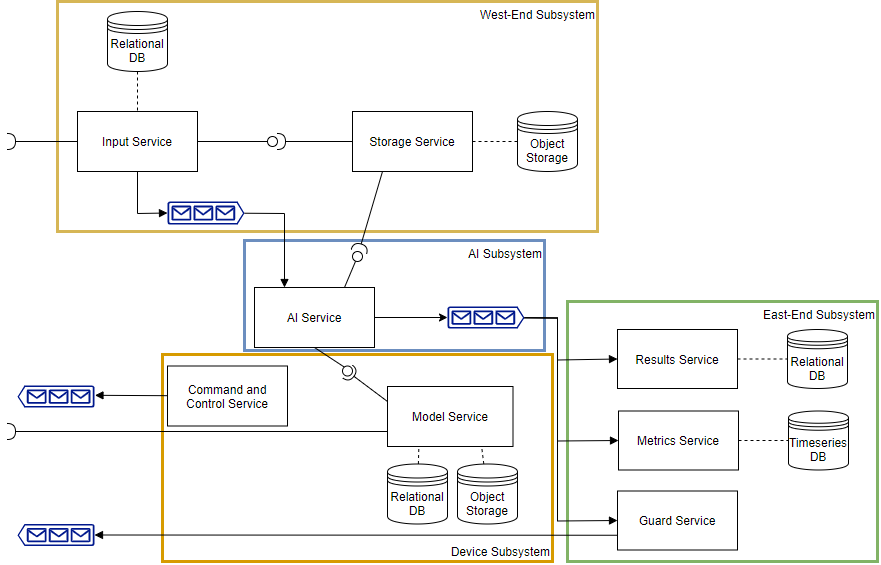
\includegraphics[width=150mm, keepaspectratio]{figures/architecture-redesigned.png}
\caption{A Birdnetes rendszer architektúrája}
\label{fig:birdnetes-components}
\end{figure}

%----------------------------------------------------------------------------
\subsubsection{IoT eszközök}
%----------------------------------------------------------------------------
Szőlőültetvényekben telepített eszközök, melyek adott időközönként publikálják állapotaikat egyéb metaadatokkal egy üzenetsoron.
Emellett folyamatosan hangfelvételt készítenek a beépített mikrofonjaikkal, mely hangfelvételekről egy másik belső szenzor eldönti,
hogy érdemes-e felküldeni a rendszerbe, ha igen, akkor egy másik üzenetsoron publikálják ezeket a hangfelvételeket.
Tartalmaznak még egy hangszórót is, mely a madarak elijesztését szolgálja.

%----------------------------------------------------------------------------
\subsubsection{Input Service}
%----------------------------------------------------------------------------
A kihelyezett IoT eszközök által felvett hangfájlok ezen a komponensen keresztül érkeznek be a rendszerbe.
Itt történik a hanganyaghoz tartozó metaadatok lementése az Input Service saját adatbázisába. 
Ilyenek például a beküldő eszköz azonosítója, a beérkezés dátuma vagy a hangüzenet rendszerszintű egyedi azonosítója.
Amint a szolgáltatás a berékezett üzenettel kapcsolatban elvégezte az összes feladatát, 
publikál egy üzenetet az MQTT üzenetsorra a többi kliensnek feldolgozásra.

%----------------------------------------------------------------------------
\subsubsection{AI Service}
%----------------------------------------------------------------------------
Az AI Service példányai fogadják az Input Service-től érkező üzeneteket és elkezdik klasszifikálni az abban található hanganyagot.
Meghatározzák, hogy a hanganyag mekkora valószínűséggel volt seregély hang vagy sem.
Ennek eredményét a hangminta egyedi azonosítójával együtt publikálják egy másik üzenetsoron.

%----------------------------------------------------------------------------
\subsubsection{Guard Service}
%----------------------------------------------------------------------------
A Guard Service feliratkozik az AI Service által publikált üzenetek témájára 
és valamilyen valószínűségi kritérium alapján eldönti, hogy a hangminta tartalmaz-e seregély hangot.
Ha igen, akkor az üzenetsoron küld egy riasztás parancsot a hanganyagot küldő eszköznek.

%----------------------------------------------------------------------------
\subsubsection{Command and Control Service}
%----------------------------------------------------------------------------
A Command and Control Service az előzőekkel ellentétben egyáltalán nem vesz részt a minták fogadásában, feldolgozásában vagy kezelésében.
Felelősége az eszközök és azok szenzorai állapotának menedzselése és követése.
Ezen keresztül lehet az egyes eszközöket ki- és bekapcsolni.

% List of Figures, Tables
%~~~~~~~~~~~~~~~~~~~~~~~~~~~~~~~~~~~~~~~~~~~~~~~~~~~~~~~~~~~~~~~~~~~~~~~~~~~~~~~~~~~~~~
%\listoffigures\addcontentsline{toc}{chapter}{\listfigurename}
%\listoftables\addcontentsline{toc}{chapter}{\listtablename}


% Bibliography
%~~~~~~~~~~~~~~~~~~~~~~~~~~~~~~~~~~~~~~~~~~~~~~~~~~~~~~~~~~~~~~~~~~~~~~~~~~~~~~~~~~~~~~
\addcontentsline{toc}{chapter}{\bibname}
\bibliography{bib/mybib}


% Appendix
%~~~~~~~~~~~~~~~~~~~~~~~~~~~~~~~~~~~~~~~~~~~~~~~~~~~~~~~~~~~~~~~~~~~~~~~~~~~~~~~~~~~~~~
%----------------------------------------------------------------------------
\appendix
%----------------------------------------------------------------------------
\chapter*{\fuggelek}\addcontentsline{toc}{chapter}{\fuggelek}
\setcounter{chapter}{\appendixnumber}
%\setcounter{equation}{0} % a fofejezet-szamlalo az angol ABC 6. betuje (F) lesz
\numberwithin{equation}{section}
\numberwithin{figure}{section}
\numberwithin{lstlisting}{section}
%\numberwithin{tabular}{section}

%----------------------------------------------------------------------------
\section{A Docker image készítéséhez használt fájlok}
%----------------------------------------------------------------------------
\begin{lstlisting}[style=dockerfile, caption=A Dockerfile tartalma, label=lst:dockerfile]
    FROM mcr.microsoft.com/dotnet/aspnet:5.0 AS base
    WORKDIR /app
    RUN apt-get update && apt-get install -y curl
    RUN curl -sL https://deb.nodesource.com/setup_12.x | bash -
    RUN apt-get update && apt-get install -y nodejs

    FROM mcr.microsoft.com/dotnet/sdk:5.0 AS build
    RUN apt-get update && apt-get install -y curl
    RUN curl -sL https://deb.nodesource.com/setup_12.x | bash -
    RUN apt-get update && apt-get install -y nodejs
    WORKDIR /src
    COPY ["Birdmap.API/Birdmap.API.csproj", "Birdmap.API/"]
    COPY ["Birdmap.BLL/Birdmap.BLL.csproj", "Birdmap.BLL/"]
    COPY ["Birdmap.Common/Birdmap.Common.csproj", "Birdmap.Common/"]
    COPY ["Birdmap.DAL/Birdmap.DAL.csproj", "Birdmap.DAL/"]
    RUN dotnet restore "Birdmap.API/Birdmap.API.csproj"
    COPY . .
    WORKDIR "/src/Birdmap.API"
    RUN dotnet build "Birdmap.API.csproj" -c Release -o /app/build

    FROM build AS publish
    RUN dotnet publish "Birdmap.API.csproj" -c Release -o /app/publish

    FROM base AS final
    WORKDIR /app
    COPY --from=publish /app/publish .
    ENTRYPOINT ["dotnet", "Birdmap.API.dll"]
\end{lstlisting}

\begin{lstlisting}[style=docker-compose, caption=A docker-compose.yml fájl tartalma, label=lst:docker-compose]
    version: '3.4'

    services:
        db:
            image: "mcr.microsoft.com/mssql/server:2019-latest"
            environment:
              - ACCEPT_EULA=Y
              - SA_PASSWORD=RPSsql12345
    
        birdmap.api:
            image: ${DOCKER_REGISTRY-}birdmapapi
            ports:
                - "8000:80"
                - "8001:443"
            volumes:
                - ${APPDATA}/Microsoft/UserSecrets:/root/.microsoft/usersecrets:ro
                - ${APPDATA}/ASP.NET/Https:/root/.aspnet/https:ro
            build:
                context: .
                dockerfile: Birdmap.API/Dockerfile
            depends_on:
                - db
            environment:
                ...
                - Birdmap_LocalDbConnectionString=Data Source=db;Initial Catalog=birdmap;User=sa;Password=RPSsql12345
                - Birdmap_Defaults__Users__0__Name=admin
                - Birdmap_Defaults__Users__0__Password=pass
                - Birdmap_Defaults__Users__0__Role=Admin
                - Birdmap_Defaults__Users__1__Name=user
                - Birdmap_Defaults__Users__1__Password=pass
                - Birdmap_Defaults__Users__1__Role=User
                - Birdmap_Defaults__Services__Local-Database=https://localhost:8001/health
                - Birdmap_Defaults__Services__KMLabz-Service=https://birb.k8s.kmlabz.com/devices
                - Birdmap_UseDummyServices=true
                - Birdmap_ServicesBaseUrl=https://birb.k8s.kmlabz.com/
                - Birdmap_Mqtt__BrokerHostSettings__Host=localhost
                - Birdmap_Mqtt__BrokerHostSettings__Port=1883
                - Birdmap_Mqtt__ClientSettings__Id=ASP.NET Core client
                - Birdmap_Mqtt__ClientSettings__Username=username
                - Birdmap_Mqtt__ClientSettings__Password=password
                - Birdmap_Mqtt__ClientSettings__Topic=devices/output
\end{lstlisting}

%\label{page:last}
\end{document}
